\documentclass[12pt,a4paper]{article}
\usepackage[utf8]{inputenc}
\usepackage{amsmath}
\usepackage{amsfonts}
\usepackage{amssymb}

\usepackage{placeins}
\usepackage{cmap} % для кодировки шрифтов в pdf
\usepackage[T1]{fontenc}
\usepackage{hhline}
\usepackage[unicode]{hyperref}
\usepackage{multirow}
\usepackage{array}
\usepackage{amsmath}
\usepackage{bm}
\usepackage{textcomp}
\usepackage[russian]{babel}
\usepackage{graphicx} % для вставки картинок
\usepackage{amssymb,amsfonts,amsmath,amsthm} % математические дополнения от АМС
\usepackage{indentfirst} % отделять первую строку раздела абзацным отступом тоже
% Поля
\usepackage{geometry}
\geometry{left=2cm}
\geometry{right=1.5cm}
\geometry{top=2.4cm}
\geometry{bottom=2.cm}

%%%%%%%%%%%%%%%%%%%%%%%%%%%%%%%     

\linespread{1.5} % полуторный интервал
\frenchspacing




\begin{document}
	
	\begin{titlepage}
		
		\begin{center}
			\begin{large}
				Санкт-Петербургский Политехнический университет\\ Петра Великого\\
				Физико-механический институт\\
			\end{large}
			\vspace{0.2cm}
			Высшая школа прикладной математики и вычислительной физики\\
			
		\end{center}
		
		\vspace{3cm}
		\begin{center}
			\textbf{Отчёт\\ по лабораторной работе №2\\ по дисциплине\\ "Анализ данных с интервальной \\неопределенностью"}
		\end{center}
		
		\vspace{3cm}
		
		\vbox{%
			\hfill%
			\vbox{%
				\hbox{Выполнил студент:}%
				\hbox{\break}
				\hbox{Иванов Андрей Игоревич,}%
				\hbox{группа 5040102$\backslash$20201}%
				\hbox{\break}
				\hbox{\break}
				\hbox{Проверил:}
				\hbox{\break}
				\hbox{к.ф.-м.н., доцент}
				\hbox{Баженов Александр Николаевич}
			}%
		} 
		\vfill
		
		\begin{center}
			Санкт-Петербург, 2023
		\end{center}
	
	\end{titlepage}
	\tableofcontents
	\newpage
	
	\listoffigures
	\newpage
	
	\section{Постановка задачи}
            Даны четыре вещественные выборки, соответствующие показаниям -0.5, -0.25, 0.25, 0.5. Необходимо:
            \begin{itemize}
                \item Сформировать интервальную выборку по имеющимся данным.
                \item Найти точечную линейную регрессию интервальной выборки
                \item Построить информационное множество коэффициентов регрессии (решить задачу восстановления зависимости)
                \item Построить коридор совместных зависимостей задачи восстановления
            \end{itemize}
	\newpage
	
	\section{Теория}
            \subsection{Формирование интервальной выборки}
                Дано множество из N выборок вещественных чисел $\mathbf{\{X_i\}}_{i=1}^N$. По этому множеству формируется интервальная выборка по следующему принципу:
                \begin{equation}
                    X = \{(min(\mathbf{X_i}), max(\mathbf{X_i}))\ | \mathbf{X_i} \in \mathbf{\{X_i\}}_{i=1}^N \}
                \end{equation}
                
            \subsection{Точечная линейная регрессия}
                Рассматривается задача восстановления зависимости для выборки
                $ (X, \textbf(Y))$, $ X = \{x_i\}_{i=1}^{n}, \textbf{Y} = \{\textbf{y}_i\}_{i=1}^{n} $,
                $ x_i $ - точеный, $ \textbf{y}_i $ - интервальный.
                Пусть искомая модель задана в классе линейных функций:
            
                \begin{equation}
                    y = \beta_0 + \beta_1 x
                \end{equation}
            
                Поставим задачу оптимизацию для нахождения точечных оценок
                параметров $ \beta_0, \beta_1 $.
            
                \begin{equation}
                    \begin{gathered}
                        \sum_{i = 1}^{m}w_{i} \to \min \\
                        \text{mid}\textbf{y}_{i} - w_{i} \cdot \text{rad}\textbf{y}_{i} \leq \beta_0 + \beta_1 x \leq \text{mid}\textbf{y}_{i} + w_{i} \cdot \text{rad}\textbf{y}_{i} \\
                        w_{i} \geq 0, i = 1, ..., m \\
                        {w_i}, \beta_0, \beta_1 - ?
                    \end{gathered}
                    \label{e:task}
                \end{equation}
                
                Задачу можно решить методами линейного программирования.
            
                \subsection{Информационное множество}
                \textbf{Информационным множеством} задачи восстановления зависимости
                будем называть множество значений всех параметров зависимости,
                совместных с данными в каком-то смысле. 
            
                \textbf{Коридором совместных зависимостей} задачи восстановления зависимости
                называется многозначное множество отображений $ \Upsilon $, сопоставляющее
                каждому значению аргумента $ x $ множество
                
                \begin{equation}
                    \Upsilon(x) = \bigcup_{\beta \in \Omega} f(x, \beta)
                \end{equation}
                , где $ \Omega $ - информационное множество, $ x $ - вектор переменных, $ \beta $ - вектор оцениваемых параметров. 
        
	\newpage
	
	\section{Реализация}
		Лабораторная работа выполнена на языке Python 3.10 с помощью загружаемых пакетов NumPy и MatPlotLib. Исходный код лабораторной работы находится на \href{https://github.com/Drusiand/SPbSTU_Interval_Analysis.git}{GitHub репозитории}.
	\newpage
	
	\section{Результаты}

        \begin{figure}[h!]
            \centering
            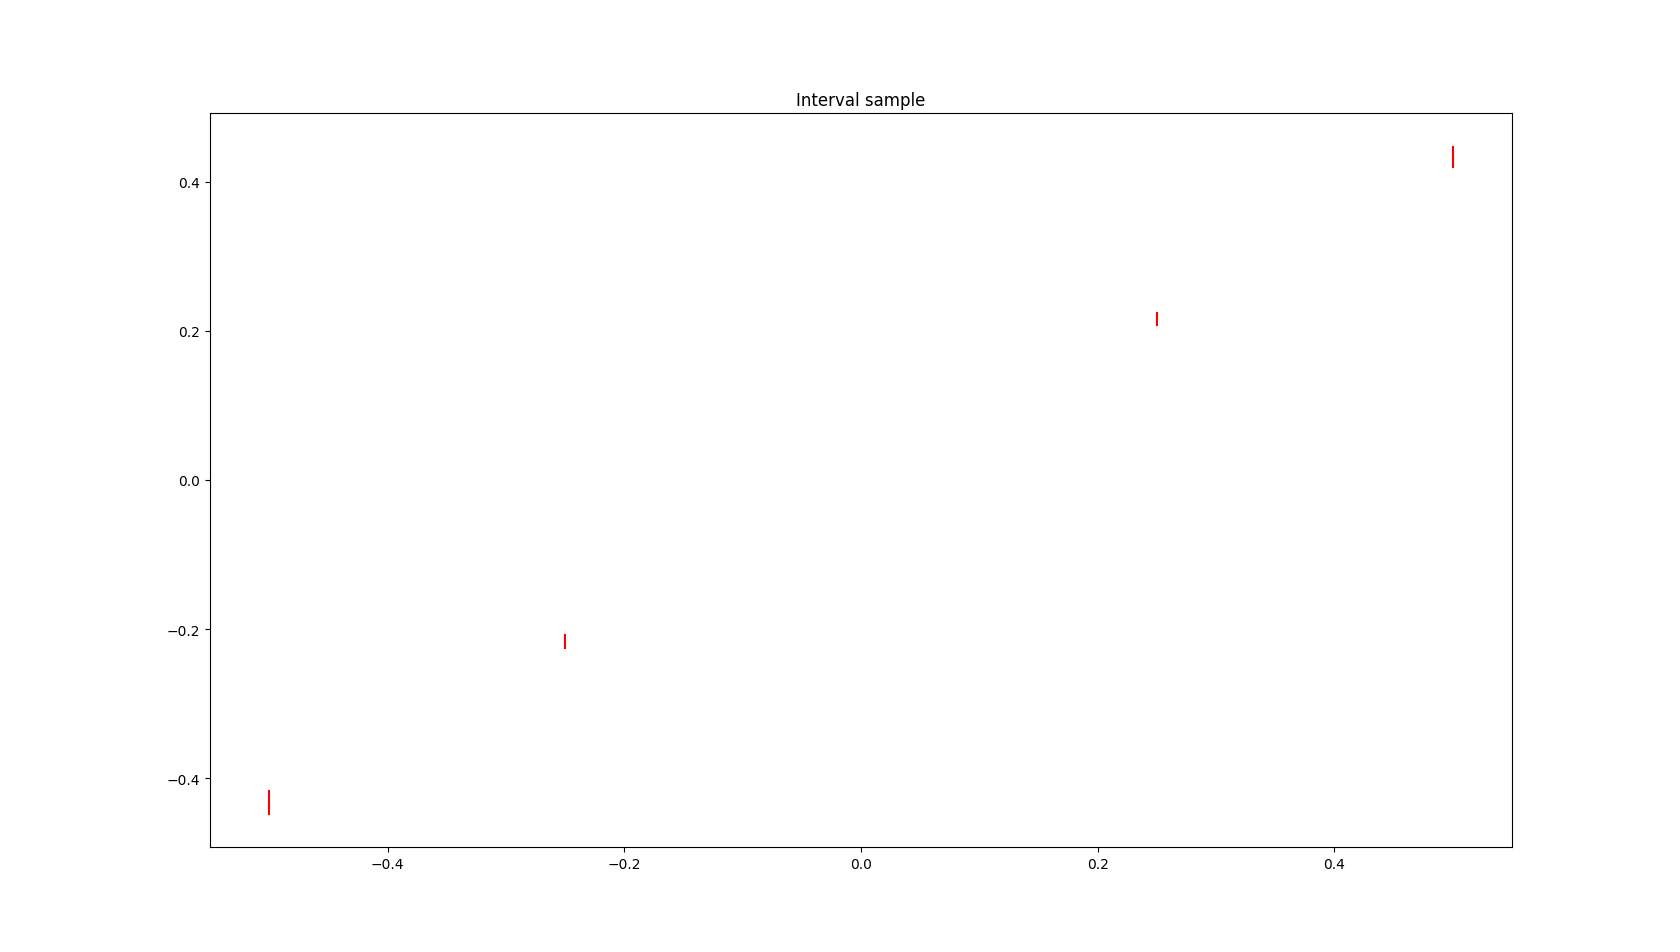
\includegraphics[width=0.95\linewidth]{sample_plot.png}
            \caption{График интервальной выборки}
        \end{figure}

        \begin{figure}[h!]
            \centering
            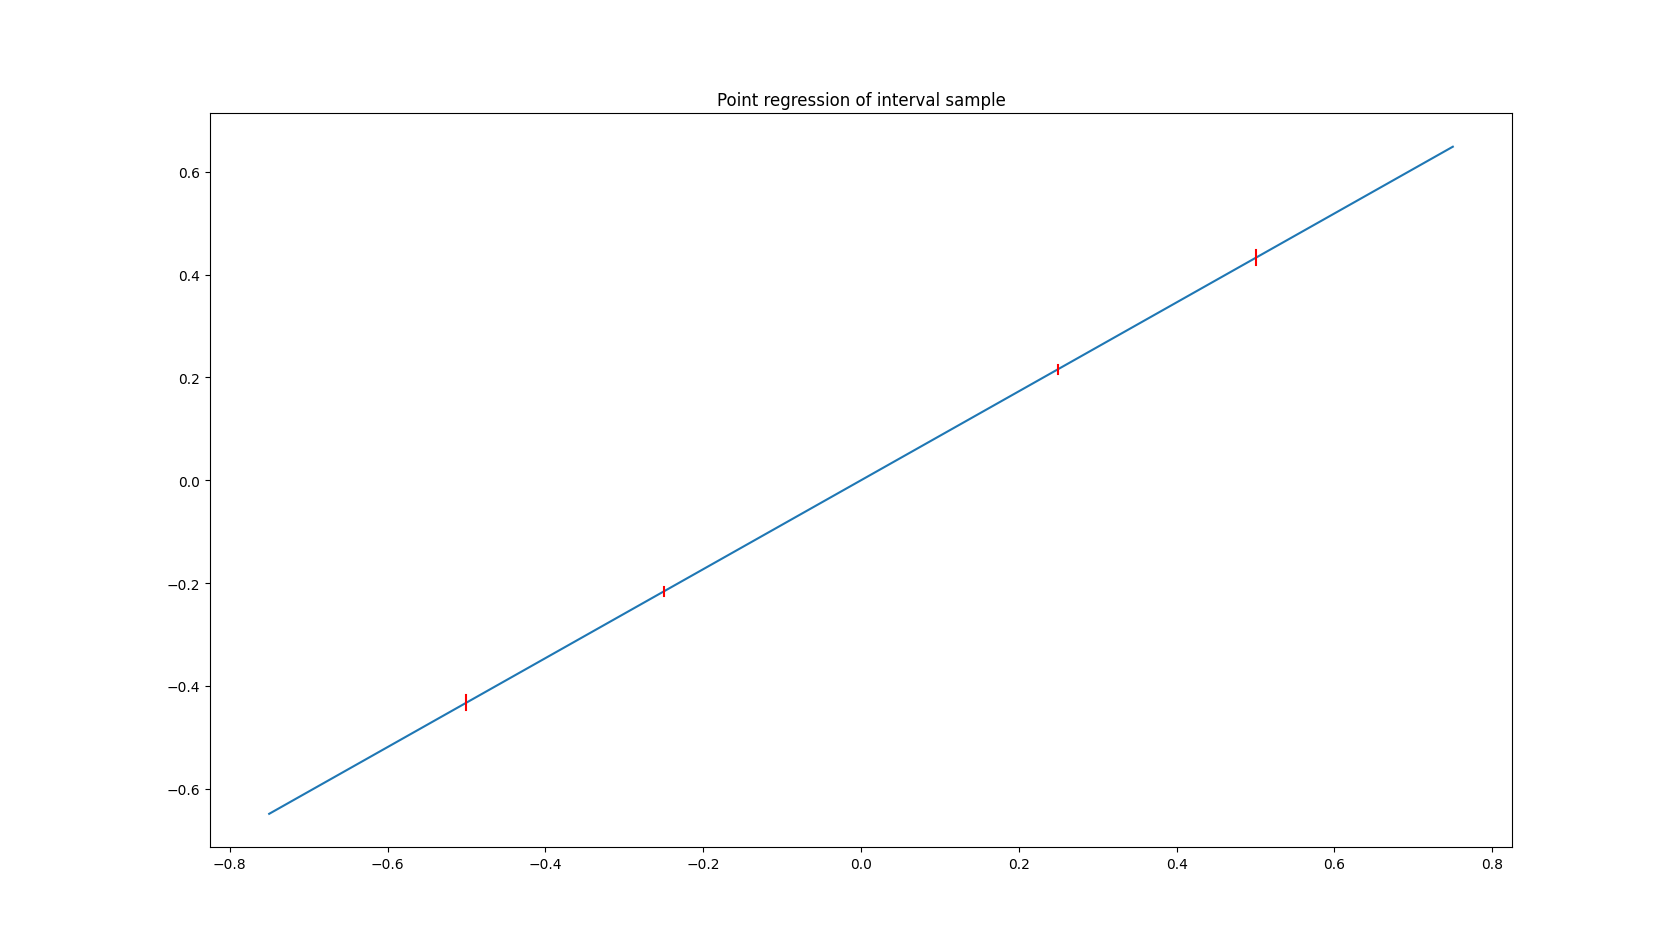
\includegraphics[width=0.95\linewidth]{sample_regr.png}
            \caption{Точечная линейная регрессия}
        \end{figure}

        \begin{figure}[h!]
            \centering
            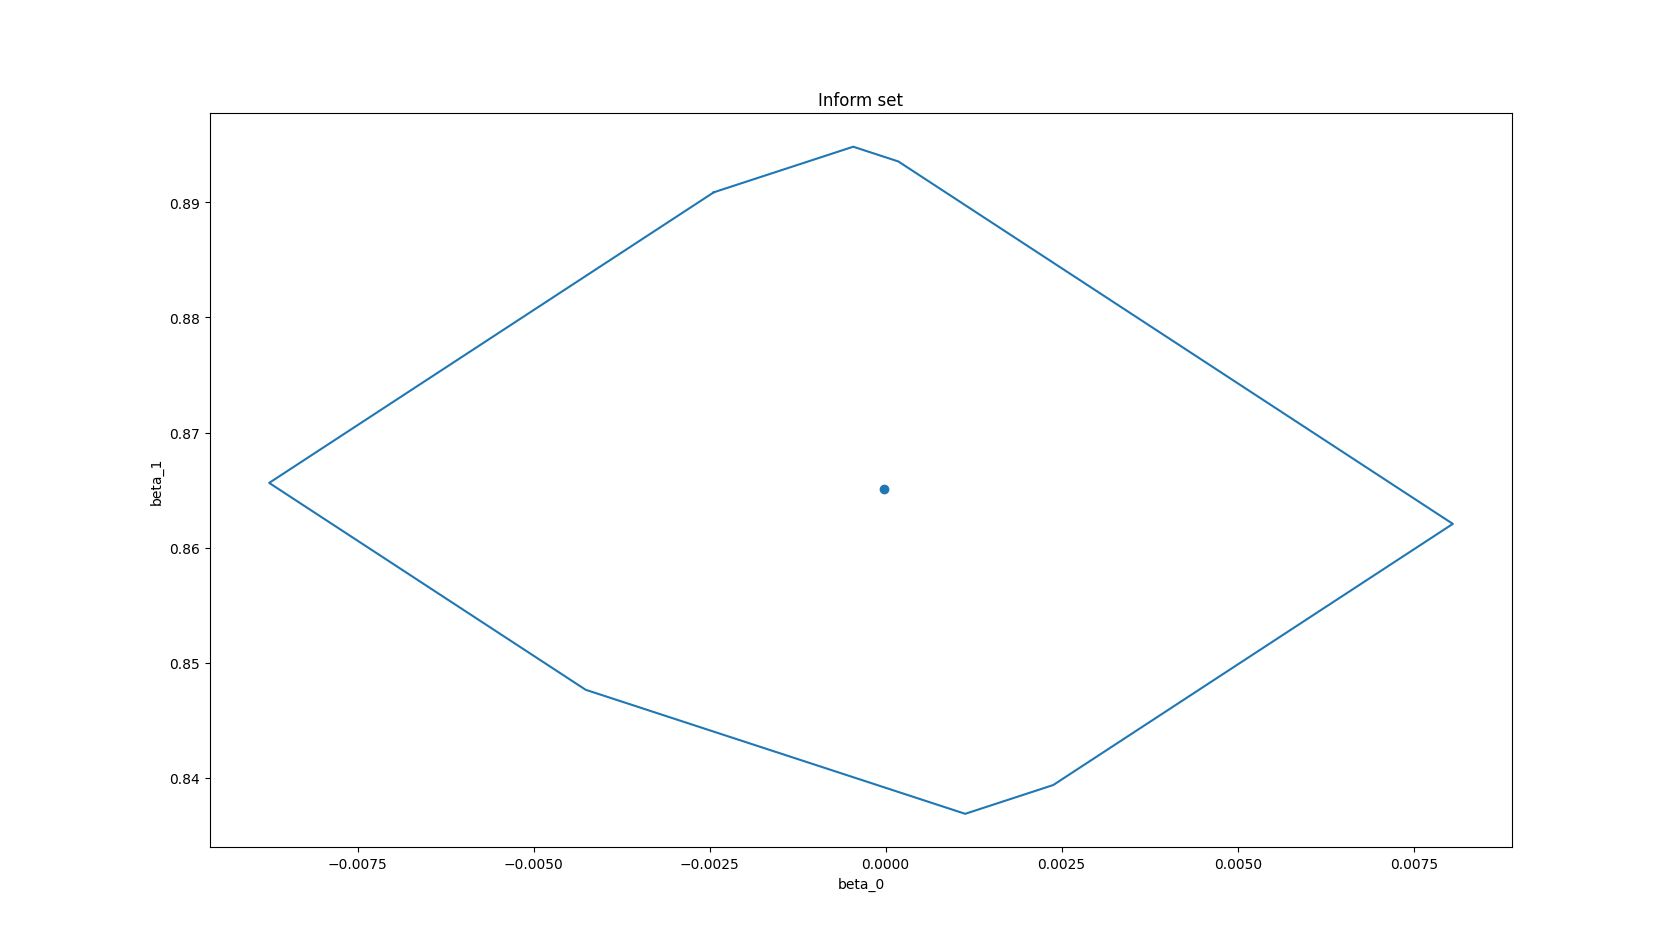
\includegraphics[width=0.95\linewidth]{sample_Inf_set.png}
            \caption{Информационное множество}
        \end{figure}

        \begin{figure}[h!]
            \centering
            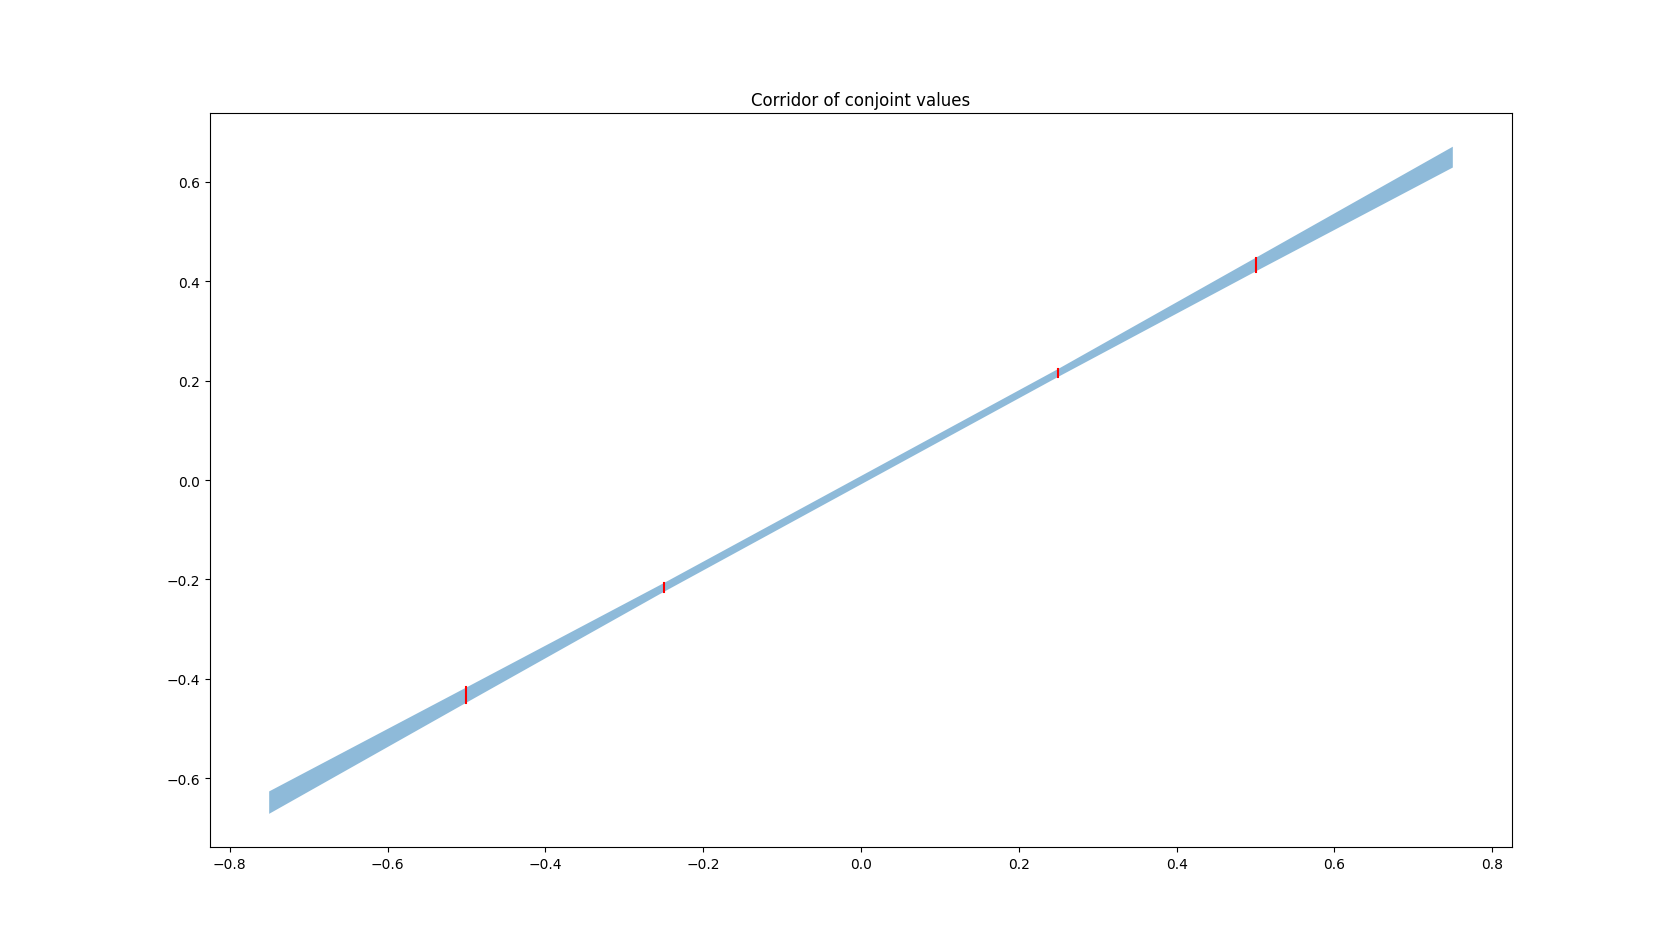
\includegraphics[width=0.95\linewidth]{sample_corrid.png}
            \caption{Коридор совместных значений}
        \end{figure}
        \FloatBarrier
        
       Ниже приведена таблица, описывающая итоговую интервальную выборку
        \begin{center}
            \begin{tabular}{|c|c|c|}
            \hline
                \textbf{Набор данных} & $\mathbf{\underline{x_i}}$ & $\mathbf{\overline{x_i}}$\\
                \hline
                -0\_5V\_4&−0.44788&−0.4173\\
                \hline
                -0\_25V\_4&−0.22516&−0.20746\\
                \hline
                0\_25V\_4&0.20765&0.22357\\
                \hline
                0\_5V\_4&0.41956&0.44696\\
                \hline
            \end{tabular}
        \end{center}
      
        Искомая модель принимает вид:
        \begin{equation}
            y = -0.00003 + 0.865112 \cdot x
        \end{equation}
        
        \clearpage
	\newpage

\end{document}